
Drone à géométrie variable
\textit{Inspiré de la thèse de Valentin RIVIERE,
” Vers un robot aérien autonome bio­inspiré à morphologie variable ”,
Thèse de doctorat en Sciences du Mouvement Humain, Aix-­Marseille, 2019}

\section*{Présentation générale}


Ce sujet porte sur la conception d’un drone quadrirotor bio­inspiré, développé à l’institut des
sciences du mouvement. Ce drone s’inspire de l’oiseau et possède la capacité de se replier
en vol afin de diminuer son envergure (\autoref{fig:01} et \autoref{fig:02}).

En fin de repliement, les bras supportant les moteurs et hélices s’alignent le long du corps
du drone pour éviter que les hélices ne touchent les bords de l’ouverture.

Cette particularité est intéressante pour des problématiques d’évitement d’obstacles dans
des milieux encombrés. Le drone est de plus pourvu d’un algorithme d’estimation de taille
d’obstacles en vol grâce à une perception visuelle monoculaire. Cet algorithme permet de
rendre le drone plus autonome pour éviter les collisions avec son environnement et actionner
son système de changement de forme si cela est nécessaire.

Tout cet ensemble consititue la plateforme Quadmorphing.


\begin{minipage}[c]{.48\linewidth}
\begin{figure}[H]
\centering
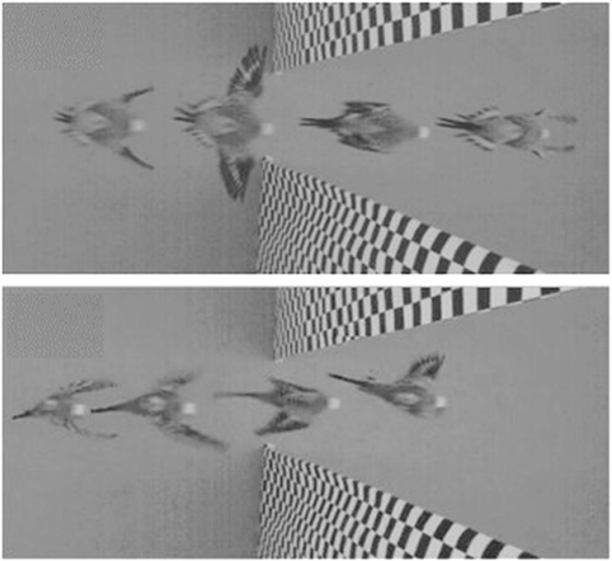
\includegraphics[width=.8\linewidth]{fig_01}
\caption{\label{fig:01} L’oiseau s’adapte au passage
plus étroit en modifiant son envergure}
\end{figure}
\end{minipage}\hfill
\begin{minipage}[c]{.48\linewidth}
\begin{figure}[H]
\centering
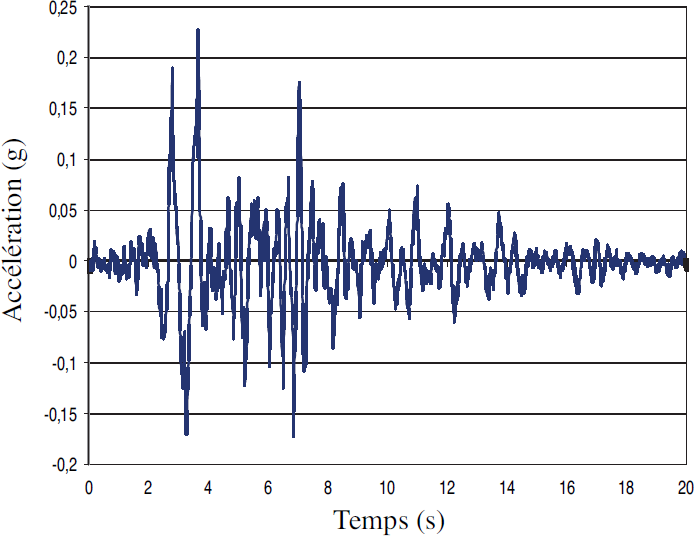
\includegraphics[width=.8\linewidth]{fig_02}
\caption{\label{fig:02} Vue CAO de la plateforme QuadMorphing passant à travers une ouverture}
\end{figure}
\end{minipage}

L'objectif de cette étude est de concevoir et valider les solutions technologiques retenues
pour la plateforme QuadMorphing permettant le passage d’ouverture en vol. Le diagramme
partiel des exigences liées à cette étude est donné en \autoref{fig:21} de l’annexe 1.
La démarche proposée est définie ci­-après :
\begin{itemize}
\item ­\autoref{sec:01} --­ influence des mouvements des bras du drone sur son comportement;
\item ­\autoref{sec:02} --­ choix d’un mécanisme de modification de l’envergure;
\item ­\autoref{sec:03} --­ analyse simplifiée de l’asservissement en roulis du drone.
\end{itemize}


\section{\label{sec:01} Influence des mouvements des bras du drone sur son comportement}

ndépendamment de la solution retenue pour mettre en mouvement les bras supportant les
moteurs et hélices, nous nous intéressons dans cette partie aux conséquences des mouvements des bras sur le comportement dynamique du drone afin de valider les choix retenus
par la suite.

\subsection{Influence de la rotation des bras sur l’envergure ­ vérification des exigences Id 1
et Id 1.1}

Pour diminuer l’envergure, on choisit de replier les bras supportant les moteurs et hélices du
drone. Le repliement doit être rapide et de courte durée. En effet, pour des raisons de contrôle
et de stabilité, il est impossible d’utiliser un drone avec les bras repliés en permanence. La
\autoref{fig:23} de l’annexe 2 présente un modèle géométrique simplifié du drone pour lequel le
bras 1, supportant les deux moteurs et hélices avant, peut tourner par rapport au corps \textbf{0} du
drone. Le bras \textbf{2}, supportant les deux moteurs et hélices arrière, peut également tourner par
rapport au corps \textbf{0}. Aussi pour cette étude d’envergure, l’analyse portera sur le bras \textbf{1} seul,
le comportement du bras \textbf{2} étant identique. La \autoref{fig:23} précise le paramétrage associé à
cette étude. L’angle de rotation du bras \textbf{1} par rapport au corps \textbf{0} du drone est noté $\gamma_1$ et peut
atteindre n’importe quelle valeur dans l’intervalle $[0\degres, 90\degres]$.
L’angle de rotation du bras \textbf{2} par rapport au corps \textbf{0} du drone est noté $\gamma_2$ et peut atteindre
n’importe quelle valeur dans l’intervalle $[90\degres, 180\degres]$.

%Q01
\question{\label{q:01} À partir de la \autoref{fig:23} de l’annexe 2, déterminer l’expression de la largeur $\ell$ en fonction de $\gamma_1$ et des données de la géométrie du drone.}
\ifprof
\begin{corrige}
\end{corrige}
\else
\fi

%Q02
\question{\label{q:02} En déduire la valeur de la réduction d’envergure $A =  1 - \dfrac{\indice{\ell}{min}}{\indice{\ell}{max}}$ et l’exprimer en \%.
Conclure sur la performance liée à l’exigence de réduction d’envergure Id 1.1.}
\ifprof
\begin{corrige}
\end{corrige}
\else
\fi


Des essais expérimentaux ont été réalisés pour analyser le passage du drone au travers
d’une ouverture carrée de taille de $\SI{20}{cm} \times \SI{20}{cm}$ et de profondeur de $\SI{1}{cm}$. L’ouverture est placée verticalement par rapport au sol et un de ses côtés est orienté horizontalement
(parallèle au sol). Selon la \autoref{fig:02}, le repère $\rep{G}$ est associé à cette ouverture 
(origine $\vect{O_G}$ centrée par rapport à l’ouverture). Pour la suite, la position 
$\vect{O_G O} = x_G \vect{x_G}+y_G \vect{y_G}+z_G \vect{z_G}$
 correspond à la position du centre d’inertie $O$ du drone par rapport au repère $\rep{G}$.

On définit selon la \autoref{fig:03} et la \autoref{fig:04}, la longueur projetée $\indice{\ell}{proj}$ et la hauteur projetée $\indice{h}{proj}$ du
drone dans le plan de l’ouverture. Les bords avant gauche et arrière droit du drone sont
représentés respectivement par les points $\indice{\ell}{gauche}$ et $\indice{\ell}{droit}$. Les bords avant haut et arrière bas
du drone sont représentés respectivement par les points $\indice{h}{haut}$ et $\indice{h}{bas}$.
Ces grandeurs dépendent des dimensions du drone et de son orientation par rapport à $\rep{G}$. En
première approximation et en considérant un angle de roulis $\indice{\theta}{R}$ (rotation autour de $\axe{O}{x_0}$) nul
lors du passage de l’obstacle, la longueur projetée $\indice{\ell}{proj}$ dépend uniquement des dimensions
du drone et de l’angle de lacet $\indice{\theta}{L}$ (rotation autour de $\axe{O}{z_0}$), et la hauteur projetée hproj dépend
uniquement des dimensions du drone et de l’angle de tangage $\indice{\theta}{T}$ (rotation autour de $\axe{O}{y_0}$).


\noindent
\begin{minipage}[c]{.48\linewidth}
\begin{figure}[H]
\centering
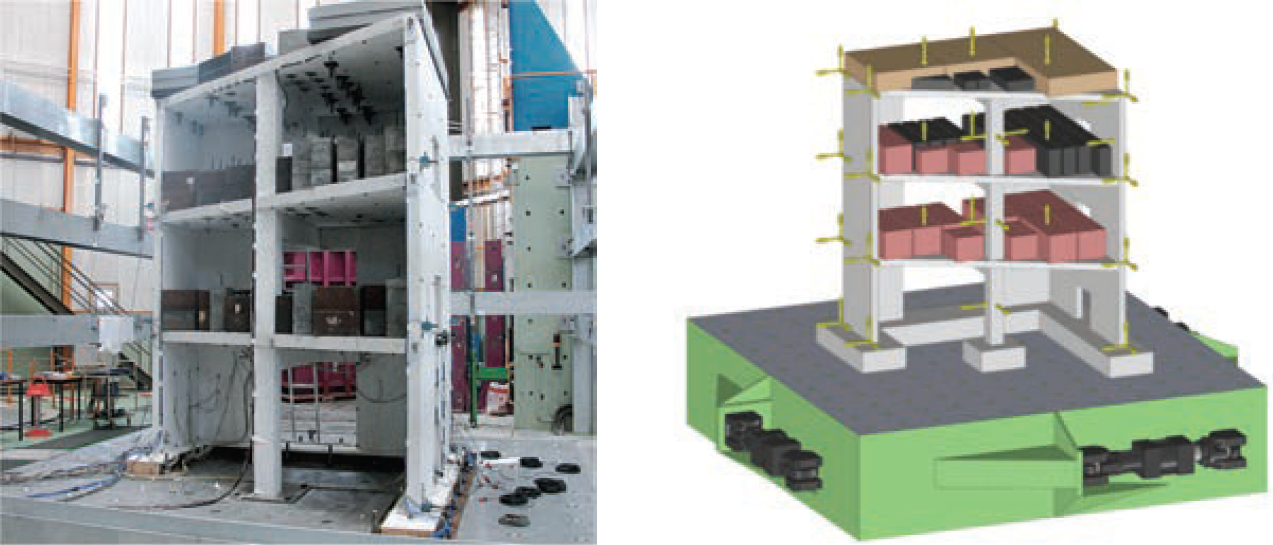
\includegraphics[width=\linewidth]{fig_03}
\caption{\label{fig:03} ­Définition de la longueur projetée $\indice{\ell}{proj}$ et de l’angle de lacet $\indice{\theta}{L}$}
\end{figure}
\end{minipage}\hspace{.5cm}
\begin{minipage}[c]{.48\linewidth}
\begin{figure}[H]
\centering
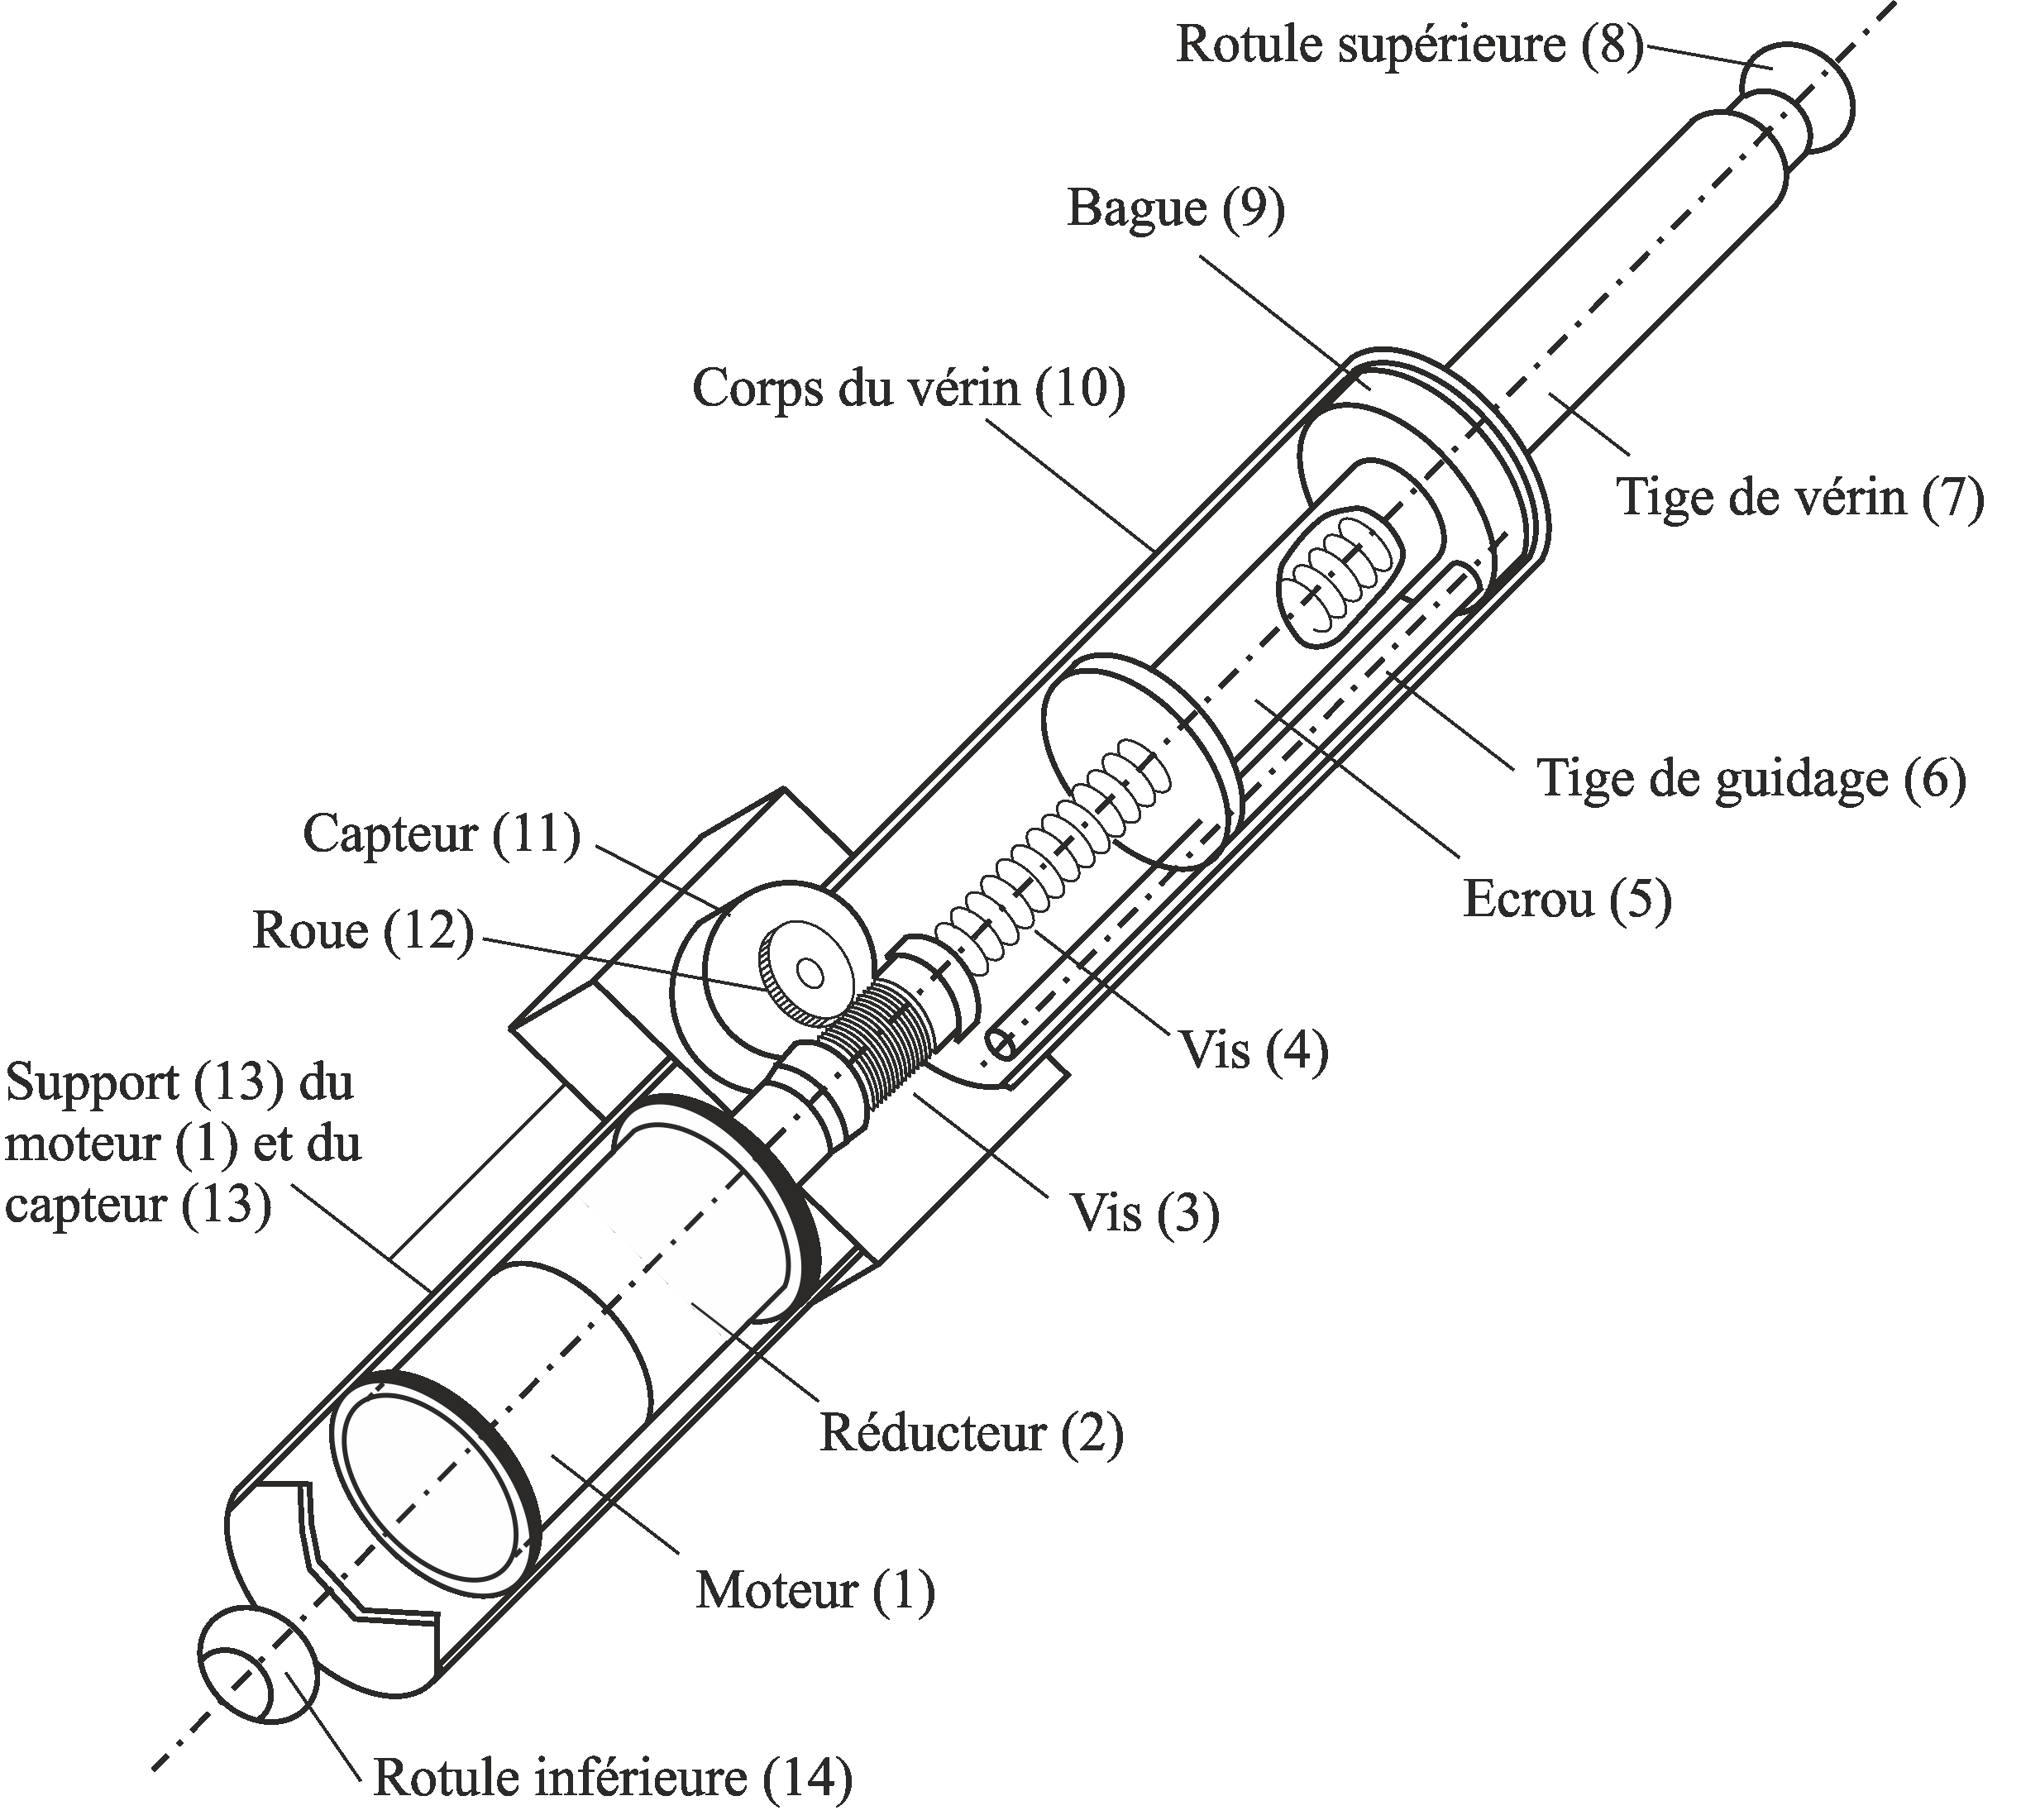
\includegraphics[width=\linewidth]{fig_04}
\caption{\label{fig:04} ­Définition de la longueur projetée $\indice{h}{proj}$ et de l’angle de lacet $\indice{\theta}{T}$}
\end{figure}
\end{minipage}

\vspace{.25cm}

Les relevés expérimentaux de 8 essais avec manœuvre de repliement des bras et passage de l’ouverture sont donnés en \autoref{fig:05}. La zone hachurée représente l’envergure de l’ouverture durant toutes les positions du robot où les collisions sont possibles, c’est­-à-­dire pour $x_G \in \left[-L/2, L/2 \right]$. L’aire grisée représente l’envergure maximale occupée par le drone durant les huit essais. Les positions des points extrêmes du drone de l’essai n°4 ($\indice{\ell}{gauche}$, $\indice{\ell}{droit}$, $\indice{h}{haut}$ et $\indice{h}{bas}$) sont représentées par les courbes avec le marqueur en forme de losange $\Diamond$. On
peut observer sur ces figures la diminution de l’envergure horizontale du drone à partir de la
consigne de repliement (représentée verticalement en pointillés à gauche). La consigne de
dépliement de la structure (représentée verticalement en pointillés à droite) est donnée dès
la sortie de la zone probable de collision afin de stabiliser le drone au plus vite.

\begin{figure}[H]
\centering
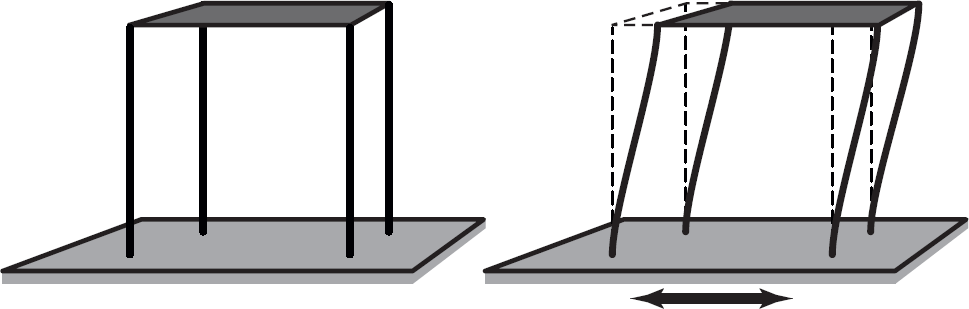
\includegraphics[width=\linewidth]{fig_05}
\caption{\label{fig:05} Vues de dessus et de côté de l’envergure du drone durant huitpassages de l’ouverture}
\end{figure}


%Q03
\question{\label{q:03}  Relever pour l’essai n°4, la valeur de $\indice{\ell}{proj}$ avant repliement (notée $\indice{\ell}{proj}^{\text{max}}$) et la comparer
à $\indice{\ell}{max}$ de la question précédente. De même pour la valeur après repliement (notée
$\indice{\ell}{proj}^{\text{min}}$) à comparer à $\indice{\ell}{min}$.
Si des écarts sont constatés entre les valeurs expérimentales et les valeurs théoriques,
expliquer l’(les) origine(s) de ces écarts.
Conclure sur la vérification de l’exigence liée au passage d’ouverture Id 1.}
\ifprof
\begin{corrige}
\end{corrige}
\else
\fi

\subsection{Influence de la rotation des bras sur la vitesse maximale en bout de pale ­-- Vérification de l’exigence Id 4}

On considère que le drone se déplace en ligne droite à la vitesse de déplacement $V_x\vect{x_0}$
selon $\vect{x_0} = \vect{x_G}$ telle que $V_x = \SI{2,5}{m.s^{-1}}$. Cette vitesse correspond à la vitesse retenue pour négocier
le passage de l’ouverture. Elle est suffisamment lente pour que le drone ait le temps d’interpréter la taille de l’ouverture et de décider si elle est franchissable ou non (dans ce cas
le drone doit avoir le temps de réaliser un freinage d’urgence avant collision). Par ailleurs,
cette vitesse est suffisamment rapide pour conserver un minimum <<~d’inertie~>> lors du franchissement et permettre sa stabilisation une fois l’ouverture franchie et les bras dépliés.

La \autoref{fig:23} et la \autoref{fig:24} complètent le paramétrage. 
On suppose que le référentiel terrestre
associé à $\rep{G}$ peut être considéré galiléen. On pose de plus $\alpha = \angl{x_1}{\indice{x}{H1}}$ l’angle définissant
l’orientation de l’hélice \textbf{H1} par rapport au bras \textbf{1}.

La vitesse de rotation du bras \textbf{1} par rapport au corps \textbf{0} du drone, $\vecto{1}{\rep{0}}$, est telle que $\vecto{1}{\rep{0}} = \dot{\gamma}_1\vect{z_0}$. La valeur maximale de cette vitesse est obtenue par une rotation de 90\degres en \SI{300}{ms}.
La vitesse de rotation de l’hélice \textbf{H1} par rapport au bras \textbf{1}, $\vecto{H1}{\rep{1}}$, est telle que 
$\vecto{H1}{\rep{1}} = \omega_1\vect{z_0} = \alphap \vect{z_0}$. 
On considérera que la vitesse de rotation de l’hélice est égale à
\SI{13 400}{tr/min} pour assurer la portance et le déplacement horizontal du drone à $V_x = \SI{2,5}{m.s^{-1}}$.

%Q04
\question{\label{q:04} Déterminer l’expression littérale de $\vectv{P}{H1}{\rep{G}}$, la vitesse en bout de pale de l’hélice
\textbf{H1} par rapport à $\rep{G}$, en fonction des données et notamment de $\dot{\gamma}$ et de $\omega_1$.}
\ifprof
\begin{corrige}
\end{corrige}
\else
\fi

%Q05
\question{\label{q:05} Dans quelle configuration du bras et de la pale cette vitesse en bout de pale est­elle
maximale ?
Déterminer dans ce cas l’expression maximale de la norme, notée $\indice{V}{max}$. Réaliser l’application numérique en déterminant au préalable la valeur numérique de chacun des
termes de l’expression de $\indice{V}{max}$.
Commenter l’influence de la vitesse de rotation des bras du drone sur la valeur de
$\indice{V}{max}$ et sur la vérification de l’exigence Id 4}
\ifprof
\begin{corrige}
\end{corrige}
\else
\fi

\subsection{Influence de la rotation des bras sur le comportement dynamique du drone selon
l’axe de lacet ­ vérification de l’exigence Id 1.1.1}

On cherche à déterminer la relation à donner entre les rotations $\gamma_1$ et $\gamma_2$ des deux bras du
drone de manière à limiter les perturbations sur le comportement dynamique en vol du drone
lors des phases de repliement et dépliement. L’objectif est d’avoir un moment dynamique du
drone selon l’axe de lacet (axe $\axe{O}{z_0}$) en $O$, centre d’inertie du drone, indépendant de $\gamma_1$
et $\gamma_2$ (et de leurs dérivées successives). Les matrices d’inerties des principaux éléments du
drone, dont la géométrie a été simplifiée pour cette étude, sont données en annexe 3.

\begin{hypo}
On suppose le drone en vol rectiligne à vitesse constante et à altitude constante. Le référentiel associé au repère $\rep{0}$ lié au corps du drone peut être considéré galiléen.
Les vitesses de rotation des hélices sont telles que :
\begin{itemize}
\item $|\omega_1|=|\omega_2|=\omega$ constante,
\item $|\omega_3|=|\omega_4|=\omega'$ constante.
\end{itemize}
Les bras sont en phase de repliement ou dépliement, 
donc $\gamma_1 \in ]0\degres, 90\degres]$, 
$\dot{\gamma}_1 \neq 0$ et  $\ddot{\gamma}_1 \neq 0$ pour le bras \textbf{1};
idem pour les dérivées de l’angle $\gamma_2$ du bras \textbf{2}.
\end{hypo}


\begin{obj}

\end{obj}




\begin{figure}[H]
\centering
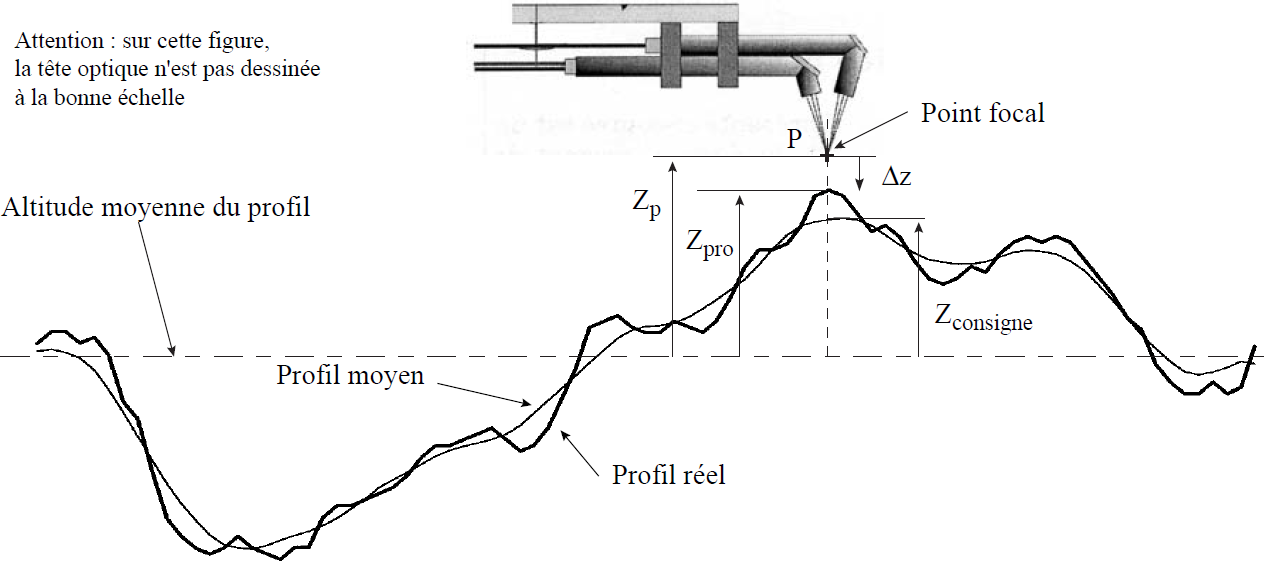
\includegraphics[width=.8\linewidth]{fig_08}
\caption{\label{fig:08}  Images en position nominale et décalée}
\end{figure}


%Q18
\question{\label{q:19}}
\ifprof
\begin{corrige}
\end{corrige}
\else
\fi


